\chapter{Contributions}
	The general contribution of the thesis is a safety-critical design approach that employs formal methods at various stages of software development such as requirements specification and software design, and a power-efficient and integrated mapping of the software to hardware while satisfying timing and reliability of the software in a distributed environment. It satisfies the research goals explained in Section x via the specific contributions: a requirements specification editor~\cite{Mahmud2015ReSA:Systems}\cite{resatool}, a formal analysis of the specifications~\cite{resatool}\cite{Mahmud2017SpecificationLogic}, a formal analysis of Simulink models~\cite{Filipovikj2018SimppaalModels} and optimization of software mappings in the context of distributed architecture~\cite{Mahmud5222}\cite{Mahmud2019Power-awareOptimization}. The contributions are contextualized in a development framework that make use of EAST-ADL, AUTOSAR and Simulink, as illustrated by the workflow diagram shown in Figure~\ref{fig_workflow}.
\begin{figure}[h]
	\centering
	\ifpdf
	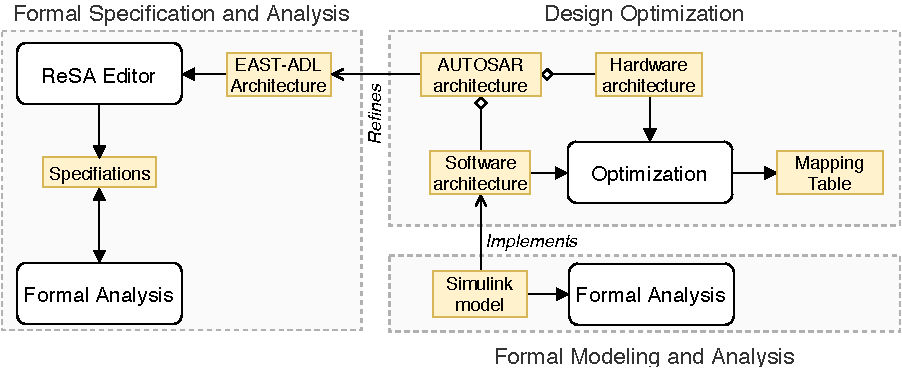
\includegraphics[width=\linewidth]{images/approach_workflow}
	\else
	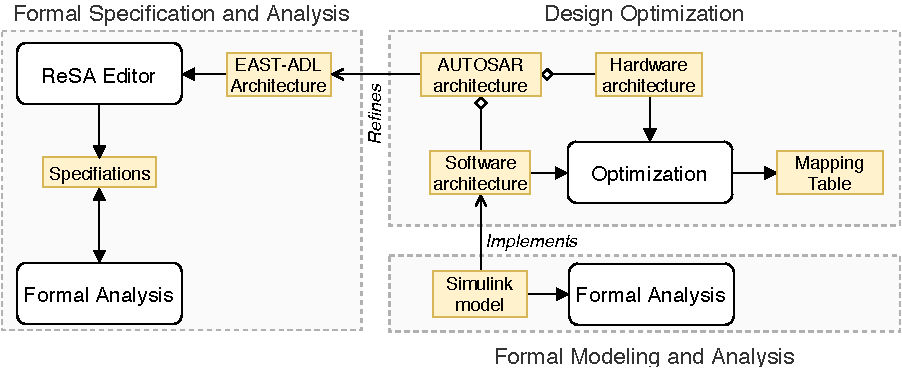
\includegraphics[width=.8\linewidth]{images/approach_workflow.eps}
	\fi
	\caption{Thesis contributions workflow.} 
	\label{fig_workflow}
\end{figure}

Initially requiremens are specified in our domain-specific language ReSA, which is a constrained natural language, by accessing model elements from an EAST-ADL architecture. The specification, which supports rudimentrary syntax and type checking, is followed by formal analysis of the specifications such as to detect and remove logicalinconsistencies. We assume the software design is implemented (or modeled) in Simulink, subsequently, Simulink models are formally analyzed against the specifications. Finally, the software functionality is mapped to the underlying hardware architecture which considers optimizing power consumption while meeting timing and reliability constraints of a distributed safety-critical software, modelin in AUTOSAR.

\section{ReSA - a Requirements Specification Language}
The language is designed to improve comprehensibility and reduce ambiguity of embedded systems specifications. It is a constrained natural language on both syntax and semantic levels. There are fixed syntactic rules to construct valid statements, and embedded system concepts that dectate the semantic construction of statements as shown in Table x, and relations between instances of the concepts.
% Please add the following required packages to your document preamble:
% \usepackage{booktabs}
\begin{table}[]\small
	\begin{tabular}{@{}lp{0.8\textwidth}@{}}
		\toprule
		Concept & Description \\ \midrule
		System & refers to any physical or logical entity that can process an input and return an output, e.g., the Adjustable Speed Limiter system, Cruise-control system \\
		Parameter & refers to the input and output parameters of a system, e.g., vehicle speed, vehicle speed set by the driver, torque force, etc. \\
		Device & the input and output devices of a system, e.g., sensors and actuators, human-machine interfaces, etc. \\
		State & refers to the operational and dynamic state of a system and its components, e.g., ASL activated, ASL deactivated, ASL enabled, etc. \\
		Mode & refers to the collection of operational capabilities and activities to achieve system objective, e.g.,,ASL mode,Cruise-control mode, etc. \\
		Entity & refers to internal or external occurrences that need to be handled by a system \\ \bottomrule
	\end{tabular}
\end{table}

Boilerplates ....
% Please add the following required packages to your document preamble:
% \usepackage{booktabs}
\begin{table}[]\small
	\begin{tabular}{@{}lp{0.75\textwidth}@{}}
		\toprule
		Boilerplate & Description \\ \midrule
		Simple & instantiates a simple statement, e,g., \texttt{Simple := System Verb within Quantity TimeUnit.} \\
		Compound & instantiates a compound statement, e.g., \texttt{Compound := Simple and/or {Simple}+} \\
		Complex & instantiates complex statement, and is constructed from Simple and a subordinating conjunction, such as when, while, until, e.g., \texttt{Complex := if Simple, Simple} \\
		Nested-Complex & instantiates nested-complex statements, and is constructed from independent clause and complex boilerplate(s), e.g., \texttt{Ncomplex := after Simple, Complex.} \\
		Conditional & instantiates conditional statements including if, if-else, if-else-if \\ \bottomrule
	\end{tabular}
\end{table}

Examples ...
\begin{table}[]\small
	\begin{tabular}{@{}lp{.9\textwidth}@{}}
		R1 & ASL:system shall send "the driver":user notification:status every 200ms. \\
		R2 & \begin{tabular}[c]{@{}l@{}}if (ASL:system is activated and\\
			\hspace{0.5cm}(the driver:user presses PAUSEBtn:inDevice or\\vehicle:user is not in running:mode))\\ then
			\\\hspace{0.5cm}ASL:system shall stop to limit vehicle speed:parameter and
			\\\hspace{0.5cm}ASL status:status shall be set to enabled \\ endif\end{tabular} \\
		R3 & After ASL:system is enabled, if IncButton:inDevice is pressed, ASL:system shall be activated.
	\end{tabular}
\end{table}
\section{Formal Analysis of ReSA Specifications}
The ReSA specifications are transformed into Boolean and propositional logics to conduct rogorous analysis besides syntax and type checking such as consistency checking. The Boolean expressions are check for consistency via a SAT solver, and the description-logic specifications via an ontology enference engine. 

\subsection{SAT-based Analysis}.
specifications are translated into Boolean expressions, subsequently, an SMT solver is employed to check the consistency of the specifications. The analysis is scalable as the SAT solving scalable to thousands of propositional variables, though shallow since the details of each clause in the specifications are abstracted by a propositional variable. Thus, advanced analysis is not possible or suitable using the Boolean approach, e.g., the clauses ``ASL is activated'' and "ASL is deactivated" are represented by two variables and does not cosider the lexical relation between the `activated'' and ``deactivated'' words, which in fact are antonyms. Moreover, temporal analysis is not suitable or intractable. 

Consider the conditional requirements R2, its translation to a Boolean expression is  $(a\land(b\lor c))\rightarrow (d\land e)$, where $a$ is ``ASL:system is activated'', $b$ the driver:user presses PAUSEBtn:inDevice, $c$ ``vehicle:user is not in running:mode'', $d$ ``ASL:system shall stop to limit vehicle speed:parameter'', $e$ ``ASL status:status shall be set to enabled''.

\subsection{Ontology-based Analysis}
The antonym relation and other lexical relations, e.g., similarity, generality, specialization, etc, can be leveraged to detect complex logical inconsistencies. So, the translation of ReSA specifications to description logic considers the lexical relations of words in statements to realizes the advanced anlalysis. Essentially, the translated specifications in the description logic constitute a requirments specification ontology, subsequently checked for consistency via an enference engine (o reasoner).

Figure x shows architecture of the requirement specification analysis using the SMT solving and ontology. 

\section{Formal and Scalable Analysis of Simulink Models}
A Simulink model consists of functional blocks, which are modeling elements to realize some functionlity, e.g., generate signal, delay a signal, mathematical operations over signals, etc., and lines connecting the blocks. The Simulink block can be either discrete or continuous depending on the block's execution behavior. If the block is executed periodically with a sample time $t_s$, it is descrete, otherwise, it is continuous if it has no sampling time, rather executes over finitely small (or minor) sampling times. The blocks can also be classified into atomic and composite blocks, where the atomic blocks, e.g., a delay block, is atomic schedulable entity that cannot be decomposed further. Whereas, the composite blocks, e.g., the Subsystem block, contains atomic blocks, and is used to create hierarchy, hence improving the visualization or to impose collective execution behavior over a set of atomic blocks. 
\paragraph{Syntax of a Simulink block}
\paragraph{Semantics of Simulink block}
The Simulink model is transformed into a network of stochastic automata, which is a formal model, using \textit{stochastic timed-automata transformation} patterns, before anlyzing the latter model via a statistical model checking. 

\subsection{Stochastic Timed Automata Transformation Patterns}
The stochastic timed-automata are continuous and descrete timed automata patters which model the generic execution behavior of the descrete and continuous blocks, respectively, thus providing a generic formalization template of Simuink models.
\begin{figure}[] 
	\centering
\subfloat[Continuous.\label{fig_continuous}]{% 
	\includegraphics[width=0.5\textwidth]{images/Continuous}
} ~
\subfloat[Discrete.\label{fig_discrete}]{% 
	\includegraphics[width=0.5\textwidth]{images/Continuous} 
} 
\caption{STA transformation pattersn.} 
\end{figure}

\subsection{Simulink Models Transformation }

\section{Fault-tolerant AUTOSAR Allocation}
\section{Scalable Fault-tolerant AUTOSAR Allocation }
\section{Validation On Industrial Use Cases}
